\documentclass[11pt,table]{beamer}
\mode<presentation>
\usepackage{etex}
\usepackage{graphicx}
\usepackage{epstopdf}
\usepackage[english]{babel}
\usepackage{tabularx}
\usepackage{booktabs}
\usepackage{mathrsfs}
\usepackage{multicol}
\usepackage{bm}
\usepackage{subcaption}
\usepackage{wrapfig}
\usepackage{dcolumn}
\usepackage{threeparttable}
\usepackage{booktabs}
\usepackage{bbm}
\usepackage{amsmath,dsfont,listings}
\usepackage{amssymb}
\usepackage{rotating}
\usepackage{multirow}
\usepackage{tcolorbox}
\usepackage[authoryear]{natbib}
\usepackage{circledsteps}
\usepackage{qtree}
\usepackage{algorithm}
%\usepackage{algorithmic}
\usepackage{algpseudocode}

\usepackage{tikz}
\usetikzlibrary{arrows,decorations.pathmorphing,backgrounds,fit,positioning,shapes.symbols,chains}
\setbeamertemplate{section in toc}[sections numbered]
\setbeamertemplate{caption}[numbered]

\bibliographystyle{Econometrica}

\setbeamersize{text margin right=3.5mm, text margin left=7.5mm}  % text margin
\setbeamersize{sidebar width left=0cm, sidebar width right=0mm}
\setbeamertemplate{sidebar right}{}
\setbeamertemplate{sidebar left}{}

\definecolor{text-grey}{rgb}{0.45, 0.45, 0.45} % grey text on white background
\definecolor{bg-grey}{rgb}{0.66, 0.65, 0.60} % grey background (for white text)
\definecolor{fu-blue}{RGB}{0, 51, 102} % blue text
\definecolor{fu-green}{RGB}{153, 204, 0} % green text
\definecolor{fu-red}{RGB}{204, 0, 0} % red text (used by \alert)
\definecolor{BrewerBlue}{HTML}{377EB8} % Define Brewer Blue
\definecolor{BrewerRed}{HTML}{E41A1C}  % Define Brewer Red

\setbeamertemplate{frametitle}{%
    \vskip-30pt \color{text-grey}\large%
    \begin{minipage}[b][23pt]{\textwidth}%
    \flushleft\insertframetitle%
    \end{minipage}%
}

\setbeamertemplate{navigation symbols}{} 

%%% begin title page
\setbeamertemplate{title page}{
\vskip2pt\hfill
\vskip19pt\hskip3pt

% set the title and the author
\vskip4pt
\parbox[top][1.35cm][c]{11cm}{\LARGE\color{text-grey} \textcolor{red1}{RL}earning:\\[1ex] \inserttitle \\[1ex] \small \quad \\[3ex]}
\vskip17pt
\parbox[top][1.35cm][c]{11cm}{\small Unit 4-4: \insertsubtitle \\[2ex] \insertauthor \\[1ex]}
}
%%% end title page

%%% colors
\usecolortheme{lily}
\setbeamercolor*{normal text}{fg=black,bg=white}
\setbeamercolor*{alerted text}{fg=fu-red}
\setbeamercolor*{example text}{fg=fu-green}
\setbeamercolor*{structure}{fg=fu-blue}

\setbeamercolor*{block title}{fg=white,bg=black!50}
\setbeamercolor*{block title alerted}{fg=white,bg=black!50}
\setbeamercolor*{block title example}{fg=white,bg=black!50}

\setbeamercolor*{block body}{bg=black!10}
\setbeamercolor*{block body alerted}{bg=black!10}
\setbeamercolor*{block body example}{bg=black!10}

\setbeamercolor{bibliography entry author}{fg=fu-blue}
\setbeamercolor{bibliography entry journal}{fg=text-grey}
\setbeamercolor{item}{fg=fu-blue}
\setbeamercolor{navigation symbols}{fg=text-grey,bg=bg-grey}
%%% end colors

%%% headline
\setbeamertemplate{headline}{
\vskip30pt
}
%%% end headline

%%% footline
\newcommand{\footlinetext}{
%\insertshortinstitute, \insertshorttitle, \insertshortdate
}
\setbeamertemplate{footline}{
\vskip2pt
\hfill \raisebox{-1pt}{\usebeamertemplate***{navigation symbols}}
\hfill \insertframenumber\hspace{10pt}
\vskip4pt
}
%%% end footline

%%% settings for listings package
\lstset{extendedchars=true, showstringspaces=false, basicstyle=\footnotesize\sffamily, tabsize=2, breaklines=true, breakindent=10pt, frame=l, columns=fullflexible}
\lstset{language=Java} % this sets the syntax highlighting
\lstset{mathescape=true} % this switches on $...$ substitution in code
% enables UTF-8 in source code:
\lstset{literate={ä}{{\"a}}1 {ö}{{\"o}}1 {ü}{{\"u}}1 {Ä}{{\"A}}1 {Ö}{{\"O}}1 {Ü}{{\"U}}1 {ß}{\ss}1}
%%% end listings

\usepackage{concmath}
\usepackage{xcolor}
\definecolor{red1}{RGB}{206, 17, 38}
\definecolor{blue1}{RGB}{16, 118, 208}
\definecolor{gray1}{RGB}{117, 115, 115}
\usepackage{hyperref}


\newtheorem{proposition}{Proposition}
\newtheorem{assumption}{Definition}

\title[]{Short guides to reinforcement learning}
\subtitle[]{Policy Gradient Methods}
\author[D. Rostam-Afschar]{\textcolor{gray1}{Davud Rostam-Afschar (Uni Mannheim)}}
\date[]{\today}
\subject{Econometrics}
\renewcommand{\footlinetext}{\insertshortinstitute, \insertshorttitle, \insertshortdate}
\hypersetup{
    bookmarks=false,
    unicode=false,
    pdftoolbar=false,
    pdffitwindow=true,
    pdftitle={Reinforcement Learning for Business, Economics, and Social Sciences: \insertsubtitle},
    pdfauthor={Davud Rostam-Afschar},
    pdfsubject={Reinforcement Learning},
    pdfkeywords={reinforcement learning, Policy Gradient Methods},
    pdfnewwindow=true,
}
\def\sym#1{\ifmmode^{#1}\else\(^{#1}\)\fi}

\begin{document}

\begin{frame}[plain]
  \titlepage
\end{frame}

% --------------------------------------------------- Slide --
%\begin{frame}
	%\frametitle{Content}
	%\tableofcontents[]
%\end{frame}

\section{Introduction to Reinforcement Learning}
{
\setbeamercolor{background canvas}{bg=BrewerBlue}
\begin{frame}
\centering
\Huge
\textcolor{white}{If I nudge my policy a little, can I win more often?}
\thispagestyle{empty}
\end{frame}
}




\begin{frame}{Model-free Policy-based Methods}
  \begin{itemize}
    \item \textbf{Q-learning}
      \begin{itemize}
        \item Model-free \emph{value}-based method
        \item No explicit policy representation\\[4ex]
      \end{itemize}
    \item \textbf{Policy gradient}
      \begin{itemize}
        \item Model-free \emph{policy}-based method
        \item No explicit value function representation
      \end{itemize}
  \end{itemize}
\end{frame}

\begin{frame}{Stochastic Policy}
  Consider a stochastic policy
  \[
    \pi_\theta(a\mid s) = \mathbb{P}(a\mid s; \theta),
  \]
  parameterized by $\theta$.
  \bigskip
	
\uncover<2->{
  \textbf{Discrete actions:} SoftMax exploration
  \[
    \pi_\theta(a\mid s)
    = \frac{\exp\bigl(h(s,a;\theta)\bigr)}
           {\sum_{a'} \exp\bigl(h(s,a';\theta)\bigr)},
  \]
  where $h(s,a;\theta)$ can be
  \begin{itemize}
    \item \emph{linear} in $\theta$: $h(s,a;\theta)=\sum_i \theta_i f_i(s,a)$
    \item \emph{nonlinear} in $\theta$: $h(s,a;\theta)=\mathrm{NeuralNet}(s,a;\theta)$
  \end{itemize}
}
\uncover<3->{

  \bigskip
  \textbf{Continuous actions:} Gaussian
  \[
    \pi_\theta(a\mid s)
    = \mathcal{N}\bigl(a\mid \mu(s;\theta),\,\Sigma(s;\theta)\bigr).
  \]
	}
\end{frame}

\section{Stochastic Gradient Policy}
{
\setbeamercolor{background canvas}{bg=BrewerBlue}
\begin{frame}
\centering
\Huge
\textcolor{white}{Stochastic Gradient Policy}
\thispagestyle{empty}
\end{frame}
}


\begin{frame}{Supervised Learning}
  \begin{itemize}
    \item Consider a stochastic policy
  \[
    \pi_\theta(a\mid s) 
  \]
		\item Data: state–action pairs $\{(s_1,a_1^*),(s_2,a_2^*),...\}$
    \item Maximize log-likelihood of the data:
      \[
        \theta^* = \arg\max_\theta \sum_n \log \pi_\theta(a_n^*\mid s_n).
      \]
    \item Policy gradient update:
      \[
        \theta_{n+1} \leftarrow \theta_n
        + \alpha_n \,\nabla_\theta \log \pi_\theta(a_n^*\mid s_n).
      \]
  \end{itemize}
\end{frame}

\begin{frame}{Reinforcement Learning}
  \begin{itemize}
	    \item Consider a stochastic policy
  \[
    \pi_\theta(a\mid s) 
  \]
    \item Data: state–action–reward triples $\{(s_1,a_1,r_1),(s_2,a_2,r_2),...\}$
    \item Maximize expected discounted return
      \[
        \theta^*=\arg\max_\theta\sum_{n} \gamma^n \mathbb{E}_\theta[r_n \mid s_n,a_n].
      \]
    \item Stochastic policy gradient update:
      \[
        \theta_{n+1} \leftarrow \theta_n
        + \alpha_n \,\only<1>{\gamma^n G_n}\only<2->{\textcolor{red1}{\gamma^n G_n}} \,\nabla_\theta \log \pi_\theta(a_n\mid s_n),
      \]
\uncover<3->{      where $G_n = \sum_{t=0}^T \gamma^{t} r_{n+t}$.}
  \end{itemize}
\end{frame}



\begin{frame}{Stochastic Gradient Policy Theorem}

\begin{itemize}
    \item \textbf{Stochastic Gradient Policy Theorem}
\begin{tcolorbox}[colframe=black, boxrule=1pt, sharp corners]
    \begin{equation*}
        \nabla V_{\theta}(s_0) \propto \sum_{s} \mu_{\theta}(s) \sum_{a} \nabla \pi_{\theta}(a|s) Q_{\theta}(s,a)
    \end{equation*}
\end{tcolorbox}

    \item \( \mu_{\theta}(s) \): stationary state distribution when executing policy parametrized by \( \theta \)

    \item \( Q_{\theta}(s,a) \): discounted sum of rewards when starting in \( s \), executing \( a \) and following the policy parametrized by \( \theta \) thereafter.
\end{itemize}

\end{frame}





\begin{frame}{Proof of the Policy Gradient Theorem (episodic case)}
\scriptsize
\begin{align*}
\nabla V_\theta(s) \;&= \; \nabla\Bigl[\sum_{a}\pi_\theta(a\mid s)\,Q_\theta(s,a)\Bigr], \text{for all }s\in\mathcal{S} \\
\uncover<2->{%
&= \sum_{a}\Bigl[\nabla \pi_\theta(a\mid s)\,Q_\theta(s,a)\;+\;\pi_\theta(a\mid s)\,\nabla Q_\theta(s,a)\Bigr]
  \; (\text{product rule})\\[1ex]
}
\uncover<3->{%
&= \sum_{a}\Bigl[\nabla \pi_\theta(a\mid s)\,Q_\theta(s,a)\;+\;\pi_\theta(a\mid s)\nabla\sum_{s',\,r} \mathbb{P}(s',r\mid s,a)\,\bigl(r+\gamma V_\theta(s')\bigr)\Bigr]
   \\[1pt]
}
\uncover<4->{%
&= \sum_{a}\Bigl[\nabla \pi_\theta(a\mid s)\,Q_\theta(s,a)\;+\;\pi_\theta(a\mid s)\sum_{s'}\gamma \mathbb{P}(s'\mid s,a)\,\textcolor{blue1}{\nabla  V_\theta(s')}\Bigr]
   \\[1pt]
}
\uncover<5->{%
&= \sum_{a}\Bigl[\nabla \pi_\theta(a\mid s)\,Q_\theta(s,a)\;+\;\pi_\theta(a\mid s)\sum_{s'}\gamma \mathbb{P}(s'\mid s,a)\\
&
     \textcolor{blue1}{\sum_{a'}\Bigl[\nabla \pi_\theta(a'\mid s')\,Q_\theta(s',a')  \;+\;\pi_\theta(a'\mid s')\sum_{s''}\gamma \mathbb{P}(s''\mid s',a')\,\nabla V_\theta(s'')\Bigr]}\Bigr]
   \; (\text{unrolling})\\[1pt]
}
\uncover<6->{%
&= \sum_{x\in\mathcal{S}}\sum_{k=0}^{\infty}\gamma^k \mathbb{P}\bigl(s\to x,k,\pi\bigr)\;\sum_{a}\nabla\pi(a\mid x)\,Q_\theta(x,a),
}
\end{align*}
\uncover<7->{%
with $\mathbb{P}(s\to x,k,\pi)$ of transitioning from state $s$ to state $x$ in $k$ steps under policy $\pi$.
}
\end{frame}





\begin{frame}{Proof of the Policy Gradient Theorem (episodic case)}

\begin{align*}
\nabla V_\theta(s_0) \;&= \; \textcolor{blue1}{\sum_{x\in\mathcal{S}}\sum_{k=0}^{\infty}\gamma^k\mathbb{P}\bigl(s_0\to x,k,\theta\bigr)}\;\sum_{a}\nabla\pi_\theta(a\mid x)\,Q_\theta(x,a)\\
\uncover<2->{&\propto \textcolor{blue1}{\sum_{s}\mu_\theta(s)}\sum_{a}\nabla \pi_\theta(a\mid s)\,Q_\theta(s,a)\,.}
\end{align*}
\end{frame}



\begin{frame}{Stochastic gradient}
\begin{align*}
\uncover<1->{%
\nabla V_{\theta} &\propto  \sum_s \mu_\theta(s)\sum_{a} \nabla \pi_{\theta}(a|s)\,Q_{\theta}(s,a) \\%
}
\uncover<2->{%
&= \only<2>{\textcolor{red1}{\mathbb{E}_{\theta}}\Bigl[\textcolor{red1}{\gamma^n}\sum_{a}Q_{\theta}(\textcolor{red1}{S_n},a)\,\nabla \pi_{\theta}(a|\textcolor{red1}{S_n})\Bigr]}%
\only<3->{\mathbb{E}_{\theta}\Bigl[\gamma^n\sum_{a}Q_{\theta}(S_n,a)\,\nabla \pi_{\theta}(a|S_n)\Bigr]} \\
}
\uncover<4->{%
&= \only<4>{\mathbb{E}_{\theta}\Bigl[\gamma^n\sum_{a}\textcolor{red1}{\pi_{\theta}(a|S_n)}\,Q_{\theta}(S_n,a)\,\frac{\nabla \pi_{\theta}(a|S_n)}{\textcolor{red1}{\pi_{\theta}(a|S_n)}}\Bigr]}%
\only<5->{\mathbb{E}_{\theta}\Bigl[\gamma^n\sum_{a}\pi_{\theta}(a|S_n)\,Q_{\theta}(S_n,a)\,\frac{\nabla \pi_{\theta}(a|S_n)}{\pi_{\theta}(a|S_n)}\Bigr]} \\
}
\uncover<6->{%
&= \only<6>{\mathbb{E}_{\theta}\Bigl[\gamma^n\,Q_{\theta}(S_n,\textcolor{red1}{A_n})\,\frac{\nabla \pi_{\theta}(\textcolor{red1}{A_n}|S_n)}{\pi_{\theta}(\textcolor{red1}{A_n}|S_n)}\Bigr]}%
\only<7->{\mathbb{E}_{\theta}\Bigl[\gamma^n\,Q_{\theta}(S_n,A_n)\,\frac{\nabla \pi_{\theta}(A_n|S_n)}{\pi_{\theta}(A_n|S_n)}\Bigr]} \\
}
\uncover<8->{%
&= \only<8>{\mathbb{E}_{\theta}\Bigl[\gamma^n\,\textcolor{red1}{G_n}\,\nabla \textcolor{red1}{\, \log \pi_{\theta}(A_n|S_n)}\Bigr]}
\only<9->{\mathbb{E}_{\theta}\Bigl[\gamma^n\,G_n\,\nabla \log \pi_{\theta}(A_n|S_n)\Bigr]}
}
\end{align*}
\only<8>{
$\quad \text{note that } Q_\theta(S_n,A_n)=\mathbb{E}_\theta[\textcolor{red1}{G_n}|S_n,A_n].$
}
\uncover<10->{%
\vspace{0.2cm}

Stochastic gradient at time step $n$:
\[
\nabla V_{\theta} \approx \gamma^n\,G_n\,\nabla \log \pi_{\theta}(A_n|S_n)
\]
}

\end{frame}


\begin{frame}{Stochastic gradient}


Stochastic gradient at time step $n$:
\[
\nabla V_{\theta} \approx \gamma^n\,G_n\,\nabla \log \pi_{\theta}(A_n|S_n)
\]
Discounted returns times direction that most increases the probability of repeating the action $A_n$ on future visits to state $S_n$.

\end{frame}


\section{REINFORCE Algorithm}
{
\setbeamercolor{background canvas}{bg=BrewerBlue}
\begin{frame}
\centering
\Huge
\textcolor{white}{REINFORCE Algorithm}
\thispagestyle{empty}
\end{frame}
}




\begin{frame}{REINFORCE: Monte Carlo Policy Gradient}
\renewcommand{\baselinestretch}{1.3}

\begin{tcolorbox}[colframe=black, boxrule=1pt, sharp corners]
\textcolor{red1}{REINFORCE$(s_0, \pi_{\theta})$}
\begin{itemize}
    \item[] Initialize $\pi_{\theta}$ to anything
    \item[] Loop forever (for each episode)
    \begin{itemize}
        \item[] Generate episode $s_0, a_0, r_0, s_1, a_1, r_1, \dots, s_T, a_T, r_T$ with $\pi_{\theta}$
        \item[] Loop for each step of the episode $n = 0, 1, \dots, T$
        \begin{itemize}
            \item[] $G_n \leftarrow \sum_{t=0}^{T-n} \gamma^{t} r_{t+n}$
            \item[] Update policy: $\theta \leftarrow \theta + \alpha \gamma^n G_n \nabla \log \pi_{\theta}(A_n | S_n)$
        \end{itemize}
    \end{itemize}
    \item[] Return $\pi_{\theta}$
\end{itemize}
\end{tcolorbox}

\end{frame}

\section{Policy Gradient Methods in Practice}
{
\setbeamercolor{background canvas}{bg=BrewerBlue}
\begin{frame}
\centering
\Huge
\textcolor{white}{Policy Gradient Methods in Practice}
\thispagestyle{empty}
\end{frame}
}

\begin{frame}{Example: Game of Go}


\begin{columns}[c]
    \column{0.6\textwidth}
    \begin{itemize}
        \item (simplified) rules:
        \begin{itemize}
            \item Two players (black and white)\\[2ex]
            \item Players alternate to place a stone of their color on a vacant intersection.\\[2ex]
            \item Connected stones without any liberty (i.e., no adjacent vacant intersection) are captured and removed from the board.\\[2ex]
            \item Winner: player that controls the largest number of intersections at the end of the game.
        \end{itemize}
    \end{itemize}

    \column{0.4\textwidth}
    \centering
    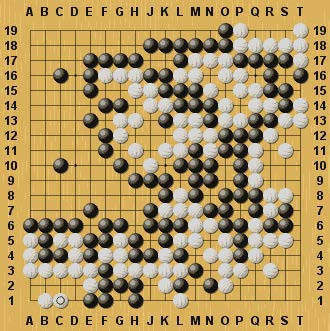
\includegraphics[width=\linewidth]{figures/1.jpg}
\end{columns}


\end{frame}



\begin{frame}{Computer Go}


\begin{columns}[c]
    \column{0.6\textwidth}
        \begin{itemize}
            \item Before: Monte Carlo Tree Search 
					\uncover<2>{
						\item Deep RL incl. policy gradient methods: AlphaGo
						}
        \end{itemize}
  
    \column{0.4\textwidth}
    \centering
    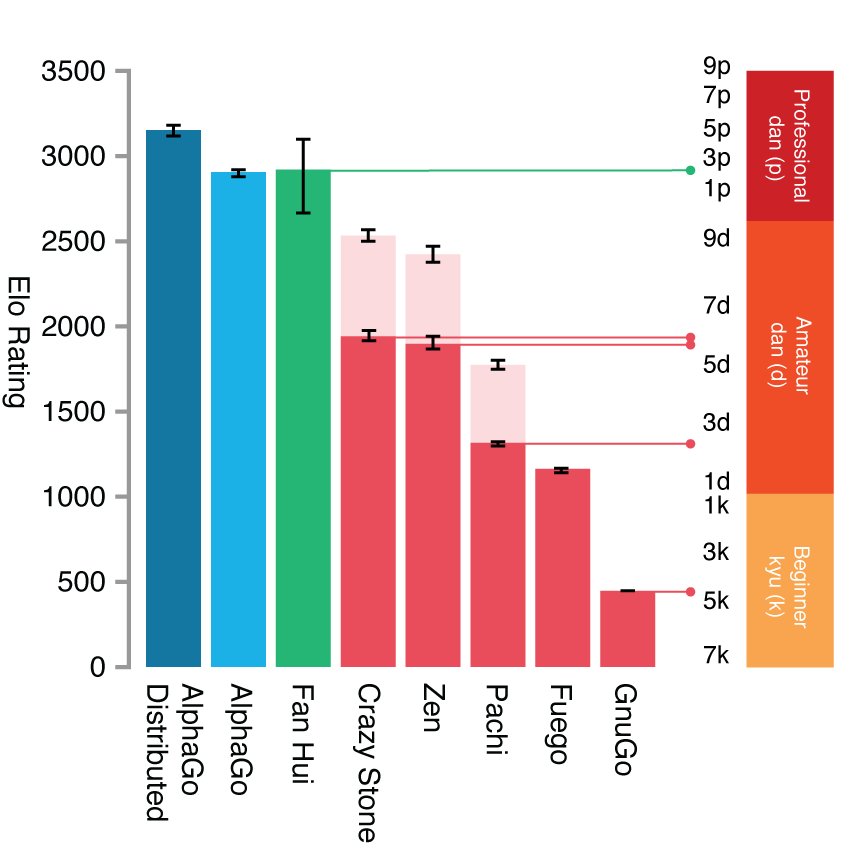
\includegraphics[width=\linewidth]{figures/2.jpg}
\end{columns}


\end{frame}

\begin{frame}{Computer Go}



\begin{itemize}
    \item March 2016: AlphaGo defeats Lee Sedol (9-dan)
    \item ``[AlphaGo] can't beat me'' --- Ke Jie (world champion)
\end{itemize}

\vspace{0.3cm}

\begin{itemize}
    \item May 2017: AlphaGo defeats Ke Jie (world champion)
\end{itemize}

\vspace{0.2cm}

\begin{itemize}
    \item ``Last year, [AlphaGo] was still quite humanlike when it played.\\
    But this year, it became like a god of Go'' --- Ke Jie (world champion)
\end{itemize}


\end{frame}



\begin{frame}[t,allowframebreaks
]\nocite{*}
\frametitle{References}
\small
\bibliography{bib}
\end{frame}
\section{Takeaways}
{
\setbeamercolor{background canvas}{bg=BrewerBlue}
\begin{frame}
\centering
\Huge
\textcolor{white}{Takeaways}
\thispagestyle{empty}
\end{frame}
}

\begin{frame}{Policy Gradient Methods}
\begin{itemize}
    \item Policy gradients directly optimize behavior to maximize rewards
    \item Stochastic policies explore actions with softmax or Gaussian distributions
    \item Good actions are reinforced by increasing their selection probability
    \item AlphaGo mastered Go by combining policy gradients, value networks, and search
\end{itemize}
\end{frame}


\end{document}
